% #######################################
% ########### FILL THESE IN #############
% #######################################
\def\mytitle{Coursework Report Part 1}
\def\mykeywords{Deadalus Delicatessen, Monster Bakery, SET08101, Bruce McClelland}
\def\myauthor{Bruce McClelland}
\def\contact{40209907@live.napier.ac.uk}
\def\mymodule{Web Technology (SET08101)}
% #######################################
% #### YOU DON'T NEED TO TOUCH BELOW ####
% #######################################
\documentclass[10pt, a4paper]{article}
\usepackage[a4paper,outer=1.5cm,inner=1.5cm,top=1.75cm,bottom=1.5cm]{geometry}
\twocolumn
\usepackage{graphicx}
\graphicspath{{./images/}}
%colour our links, remove weird boxes
\usepackage[colorlinks,linkcolor={black},citecolor={blue!80!black},urlcolor={blue!80!black}]{hyperref}
%Stop indentation on new paragraphs
\usepackage[parfill]{parskip}
%% Arial-like font
\usepackage{lmodern}
\renewcommand*\familydefault{\sfdefault}
%Napier logo top right
\usepackage{watermark}
%Lorem Ipusm dolor please don't leave any in you final report ;)
\usepackage{lipsum}
\usepackage{xcolor}
\usepackage{listings}
%give us the Capital H that we all know and love
\usepackage{float}
%tone down the line spacing after section titles
\usepackage{titlesec}
%Cool maths printing
\usepackage{amsmath}
%PseudoCode
\usepackage{algorithm2e}

\titlespacing{\subsection}{0pt}{\parskip}{-3pt}
\titlespacing{\subsubsection}{0pt}{\parskip}{-\parskip}
\titlespacing{\paragraph}{0pt}{\parskip}{\parskip}
\newcommand{\figuremacro}[5]{
    \begin{figure}[#1]
        \centering
        \includegraphics[width=#5\columnwidth]{#2}
        \caption[#3]{\textbf{#3}#4}
        \label{fig:#2}
    \end{figure}
}

\lstset{
	escapeinside={/*@}{@*/}, language=C++,
	basicstyle=\fontsize{8.5}{12}\selectfont,
	numbers=left,numbersep=2pt,xleftmargin=2pt,frame=tb,
    columns=fullflexible,showstringspaces=false,tabsize=4,
    keepspaces=true,showtabs=false,showspaces=false,
    backgroundcolor=\color{white}, morekeywords={inline,public,
    class,private,protected,struct},captionpos=t,lineskip=-0.4em,
	aboveskip=10pt, extendedchars=true, breaklines=true,
	prebreak = \raisebox{0ex}[0ex][0ex]{\ensuremath{\hookleftarrow}},
	keywordstyle=\color[rgb]{0,0,1},
	commentstyle=\color[rgb]{0.133,0.545,0.133},
	stringstyle=\color[rgb]{0.627,0.126,0.941}
}

\thiswatermark{\centering \put(336.5,-38.0){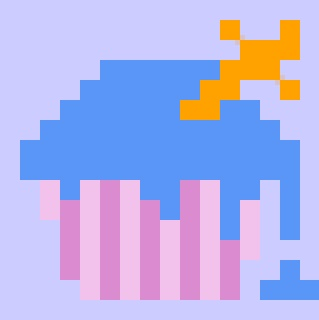
\includegraphics[scale=0.8]{logo}} }
\title{\mytitle}
\author{\myauthor\hspace{1em}\\\contact\\Edinburgh Napier University\hspace{0.5em}-\hspace{0.5em}\mymodule}
\date{}
\hypersetup{pdfauthor=\myauthor,pdftitle=\mytitle,pdfkeywords=\mykeywords}
\sloppy
% #######################################
% ########### START FROM HERE ###########
% #######################################
\begin{document}
    \maketitle
    \begin{abstract}
        This report is going to cover multiple design aspects for my game, Daedalus Delicatessen. The sections of this report cover the following; Game Descriptor, Methodologies, Features, Navigation Tree and User Interface.
    \end{abstract}
    
    \textbf{Keywords -- }{\mykeywords}
    
    \section{Game Descriptor}
	My game is a free-to-play browser based adventure-RPG where the player controls a character. They select their gender,
	name, shirt colour and starting item which will be with them until used. There will be a myriad of game changing choices.These options have an impact on future dialogue as well as game length. The game can also be reset easily if a mistake was made or just for a more wholesome experience if the player wishes to experience all it has to offer. \\
	\\
    The main aim of the game is to revert monsters back to their original human form with the legendary power of perfect baking. Ingredients can be found within the kingdom or bakery if you so wish to pick them up and there will be multiple combinations available, different coloured icings, sponges etc. Some of these options are considered bad and can cause completely different negative outcomes. A few examples of this are as follows; the monsters lunge at you, go on a rampage or even grow in size. So make sure you're polite, bake and gift them the best cake you've ever made to appease those hungry monsters.
    
	\subsection{Adventure Based Game}
	Role Playing Game (RPG) is a genre that creates incredible depth and atmosphere whilst you take control of a character(s)
	within a fictional world. There is a lot of hybrid-genres available within the mothership genre, so it is a very
	challenging genere to describe.\\
	Some sub-genres include; 
	\begin{itemize}
		\item Strategy-RPG
		\item Adventure-RPG
		\item Online-RPG
		\item Action-RPG
	\end{itemize}
	For the purpose of this report, we will talk in greater detail about text-based adventure RPGs.
	Text-based adventure RPG games have been around for a very long time. It is largely story driven
	with events unfolding when players make selections from the multiple on-screen options.
	
	\subsection{Story Draft}
	\paragraph{Daedalus Delicatessen} is a small bakery right in the center of the bustling city Cornelia. One of the only
	human populated nations in planet Terra. Monsteria is a condition that has plagued Terra since the dawn of time where
	humans turn into blood thirsty beasts, some of which call Cornelia home. Of course this caused mass panic and with skin
	several times stronger than tungsten, the royal guards are not remotely effective. \\ 
	\\
	\hspace{5mm} Child of Queen Lavender, you are a world renowned baker that makes the most delicious cakes. With the
	ancestral power to slay the stomachs of even the fiercest creatures, you are the worlds only hope to restore humankind
	to it's former glory. To do this, you need to create the most irresistable cupcakes and become Cornelias only hope!
	
	\section{Project Methodologies}
	\subsection{Javascript Game Idea}
	Javascript, HTML and CSS are all very new to me. Especially Javascript, to remedy this I decided to research how to implement all of the above in a more game type environment. As	luck would have it, I found the perfect YouTube video created by Web Dev Simplified	\cite{JavascriptGame}. This has everything I need to make a very basic game including	variables to store collected items, different ways to end the adventure (death, completion) and from the ending you can select an option to restart the game. I will use the basic format within this video to give me inspiration on how I can do my game better but with a lot more features.
	
	\subsection{Images}
	I found information on how to add images to Javascript \cite{DOMImage}. This gave me a lot of ideas on how I want to implement my images. I realized that I want to use Javascript for my images as it means that I don't need to edit the CSS every time I use an image which can adversely effect the styling on the rest of the page. This can lead to inconsistency issues within the style sheet. I also realised that there are many ways to actually implement images, these being from URLs, video frames, linking it to an image with a script and using them from the same page. The images that I will be implementing will be both static and animated. Further research led me to find a fantastic article on how to implement my ideas \cite{JavascriptImage}. I will make variables which will hold the path to my images and then use the img src tag which will contain the image dimensions as well as the file name. Images are a fantastic way to capture the players attention as it helps create a nice atmosphere, tells a vibrant story without the need to over indulge the player with a heavy text load. I will use these partnered with a descriptor for the area that they are in, the monsters, bakery etc. 
	
	\subsection{Audio} 
	I researched into multiple audio documents. HTML DOM Audio Objects \cite{DOMAudio} contained a lot of the information that I was thinking about for the project. This being automatic audio on button presses, background audio and loopable audio. Within the audio objects documentation, I found the Audio Loop page \cite{DOMAudioLoop} and the Auto Audio page \cite{DOMAudioAuto}. My reason for exploring further into these sections was due to me wanting to create the most immersive experience for the player that I possibly can. The audio will loop after a full cycle and it will play without the user doing anything to start it. This led me to wonder how I was going to go about implementing such a solution when I came across an article by Saruque Ahamed Mollick \cite{AudioAutoArticle}. This has full Javascript on how to play audio only after the page loads using window.onload. document.getElementById(audio).play() will be used to play the audio file. I will use this as inspiration to create my own.
	
	\subsection{Colour Schemes}
	I started by researching into the different colour schemes available which I found within an article by Iveta Pavlova \cite{ColourSchemes}. There were bright, dark and monochrome variants, but ultimately I decided on a softer approach, this being pastel colours. They are fun, joyful and tie in heavily with baked goods. This colour scheme symbolises part of the soft story telling that I want the player to experience. \\
	\\
    \textbf{\textit{Refer to figure 1 for the pastel colours.}} \\

	\figuremacro{h}{pastel}{Pastel Colours}{ - Family of joyful, soothing colours \cite{PastelColours}}{1.0}
  
	\subsection{Cookies and localStorage}
	Previously I had no idea how to incorporate cookies. I needed to look into the multiple ways to store data within a browser. I analysed this and found sessionStorage, localStorage and javascript cookies. I ultimately decided cookies \cite{JavascriptCookies} and localStorage \cite{LocalStorage}. This increased my understanding of the storage method in general. I am going to create cookies with document.cookies, this will be implemented to store data about the players in-game name, and character creation choices. Held items will be stored within localStorage. This will be from localStorage.setItem('BlueIcing'). This has led me to have a firmer understanding on how to store information that will be required within my website.
	
	\subsection{Favicon}
	I researched how to incorporate a favicon onto my site \cite{Favicon}. I feel that it adds a piece of my game to the tab of a browser. I will be creating my own favicon for Daedalus Delicatessen through the site favicon.cc found within 101computing.net which I linked above.

    \section{Features}
    There is a large number of different features that I will be incorporating within my game. I will go into detail about my reasoning behind these choices now. 
    
    \subsection{Player Design Choices}
    The player will input a character name of their choice, first and surname. Gender options being male, female, non-binary or alien. One of three starting bakery goods; icing, sponge or a cake casing and finally they can pick a unique colour for their shirt. All of this information will be displayed at the side of the screen. Their will be a character portrait and the players inventory alongside it so that they will know what ingredients and items they have at all times. The baked goods piece will be used to bake a cake in the future as that is one of the main components of the game. The reason I have decided to give the player so many design choices is that I believe it is what creates the most immersion and is a key factor of role-playing. Having control over multiple aspects of your character enthralls the player from the very start and makes them thirsty for more of what the game has to offer.
    
    \subsection{Data Storage}
    Cookies are stored in small text files within your browser. Normally when a web page on the server shuts down, the server forgets everything about the user. We use cookies to remedy this. I will be creating cookies using document.cookie to store all the information stated within the design choices section above, and localStorage for items found on the players journey. This primarily means that if they decide to end their adventure or that it closes by mistake, everything that they have collected up until that point will be available the next time they load up the game. Cookies and localStorage are very resilient. 
    
    \subsection{Audio}
    I will be incorporating light background audio throughout the game. Depending on players actions and the outcome of those actions, the audio will briefly change before going back to the looped audio. Audio within a game can be priceless. It sets the tonne, relaxes the player and creates the mood for the area that they are in. Studies have shown that audio within games can increase heart rate and effect respiration rate during game play \cite{In-GameAudio}. For instance, when the player or someone/thing enters the bakery, bells will ring. This adds to the atmosphere that you are visiting a shop. 
    
    \subsection{Images}
    As discussed within the research section of this report. Images are a fantastic way to capture the players attention as it helps create a nice atmosphere, tells a vibrant story without the need to over indulge the player with a heavy text load. This allows me to tell the story but also back this up with images of the monsters, the bakery and area that we are currently in. 
    
    \subsection{Multiple Paths}
    Depending on the decision that the player makes, there is going to be multiple different paths/routes to take. These decisions will lead to significantly different areas and totally different end goals. Some paths will kill you instantly, some will slow your progress and others will be the 'correct' path. I have put in such vastly differing paths as I want the player to feel like they will have to try and make the best decision that they can at the time. These decisions can lead to avoiding fights, winning fights, but this all depends on the items that you have in your inventory at the time. It will create a lot of fun atmosphere as this will really shape the game.
    
    \subsection{Columns}
    To keep the styling of the site organised, simple looking and attractive, I have opted for a multiple column, clean display with the use of flex-boxes and grids. The furthermost left column will contain the characters inventory and portrait. The center will be split into multiple sections depending on the need. Normally it will contain a box for the image a box for the text and then multiple columns for the options that are present at the bottom. This creates a fluid game space where everything you need is right in front of you in a very easy to understand format that isn't remotely cluttered. 

    \subsection{HTML Semantics}
    Semantic HTML is HTML that introduces significantly more meaning to the web page rather than just presentation. For example, a p tag indicates that the text within the element is going to be a paragraph. Compared to just putting everything within div tags, also known as Div Soup. HTML Semantics is both semantic and for the presentational values as people know what paragraphs, headings, sections, footers, headers are, and browsers know how to display them. I will be using this as it will make the different parts of the site incredibly clear to the viewers of the code as well as keeping everything neat and organised. 
    
    \subsection{Hover Effects}
    Hover Effects are a great addition that I learned how to do during week 4 whilst working on my tool bar. It is used to see which option you are hovering over in a very noticeable attractive way. The text colour is changed subtly from dark purple to black but there is also a black line above the element that you are selecting. This line expands to encompass the length of the hovered element after a second of hovering. \\
    \\
    \textbf{\textit{Refer to figure 2 for an example of my hover effect.}} \\ 
    \figuremacro{h}{hover}{Hover Effect}{ - when hovering over an element within my toolbar. This is a snipped version of my full toolbar.}{1.0} \\
    During week 4, I followed a navigation / toolbar video by Kevin Powell on Youtube \cite{Navbar}. The hover effect will make it clear which link the player is selecting in a very attractive dynamic way. It also looks very visually stimulating. 
   
    \subsection{Recipe Book}
    When the player completes a cake, the combination that they used will appear within the recipe book page. This will act like a log so that the player can feel a sense of achievement at all of the different combinations that they made. It will be tracked by the use of localStorage. 
    
    \section{Navigation Tree}
    
    \textbf{\textit{Refer to figure 3 for the navigation tree.}} \\
    \\
    \figuremacro{h}{NavigationTree}{Navigation Tree}{ - How to navigate Daedalus Delicatessen}{1.0} \\
    Using a navigation tree is a fantastic way to determine whether or not your category structures are intuitive and easy to understand. Within each of my sites, there is going to be a nav bar to travel to different sections of the website. \\
    \\
    The directory files will be structured in an easy to follow way. My main storage directory will be located within '/daedalus\_delicatessen' which I will represent as './' for the purpose of Section 5 - Navigation Tree. The './styles/styles.css' file will be attached to all of my sites, and contains the information which will control how my site looks, (headings, paragraphs, sections, div etc.) the placement and colour of the elements. Thus keeping the styles consistent throughout my website as inconsistent styles are not remotely attractive. Within the './html' directory, is 5 '"name".html' files. These files are as follows; 'index.html', 'about.html', 'game.html', 'author.html' and 'recipe\_book.html'. The game engine will be run using a javascript file and will be stored as './javascript/daedalus\_delicatessen.js'. The last directory will be './images' and contains a large volume of images. Having a centralised image store makes it much easier to use them within my '.html' files. These being the inventory images, character portraits, favicon and story images.\\
    \\
    The advantage of having such a well organised file structure is that everything is incredibly easy to find, looks significantly more professional, and is much easier to change in the future if needed.

    \section{User Interface}
    I spent a large amount of time creating my user interface using draw.io. \\
    \\
    \textbf{\textit{Refer to figure 4 for the user interface.}} \\
    \\
    I styled it with Google Chrome in mind and added the sections that are going to be within my site. I created the logo cupcake, favicon icon, inventory items and character portrait using favicon.cc and pixilart.com.
    \figuremacro{h}{interface}{User Interface}{ - Example Page During The Game.}{1.0}
    \paragraph{Pastel} - I chose this colour scheme over other colour schemes because I thought it was the most pleasant to look at, as darker schemes were too somber and neon colours were harsh on the eyes. I feel this colour scheme will work well for my game as it is joyful and enticing to the audience. \\
    The following is a list of used colours
    \begin{itemize}
		\item Body - pastel pink \#FFDDFF
		\item Navigation Bar - pastel purple \#CCCCFF
		\item Option Flex Box Divs - pastel purple \#CCCCFF
		\item Paragraph Text (all text) - dark purple \#27214F
	\end{itemize}
    As mentioned before it ties in with baked goods which will create an immersive atmosphere for the player. Finally the colour story adds a unique feel to my game, many RPG’s exist that are dark and gloomy eg ‘Skyrim’ and ‘Red Dead Redemption’. Whereas my game is light and optimistic.
    I will break each section of the site down and expand on it in detail. \\ 
    \\
    \textbf{\textit{Refer to figure 6 for the character menu.}} \\
    \paragraph{Character Menu - } This section ties in very strongly with the character design part of the game, the information will be within a section tag and then I will use 'flex-flow: column wrap' to get one on top of another. Your character name will appear just above the portrait, and the character will change clothes depending on the players clothing decision at the very start of the game. There will be 4 colour choices available. \\
    \\
    \textbf{\textit{Refer to figure 5 for the jumper colour choices.}} \\
    \figuremacro{h}{portraits}{Character Portraits}{ - the 4 jumper colour choices during the game}{1.0}
    \figuremacro{h}{interface-sidebar}{Character Menu}{ - Portrait and Inventory}{0.25} \\
    Alongside the player portrait is the characters inventory. This will contain icing, mixing bowls, spoons, casings, cakes etc. You will pick these items up throughout your adventure into the game.
    \figuremacro{h}{interface-image}{Image Location}{ - Example Story Picture}{1.0} \\
    \\
    \textbf{\textit{Refer to figure 7 for an example image.}}
    \paragraph{Story Image - }Within every section of the story, there is going to be an image which will help increase the atmosphere. These images are going to be held within img src tags, this will also contain the dimensions.
    \figuremacro{h}{interface-story}{Story Board}{ - Example Story Text and Options}{1.0}
    \paragraph{Story Board - }The story board section of my site will contain a block of text within a paragraph element. Alongside this, as stated above, the text will be dark purple \#27214F and also within a section and div tag. I am planning on making the HTML very semantic to improve readability when looking through the code and having an understanding of what items should be in what tags. 
    \paragraph{Buttons - }These options will be displayed by using a grid within my style sheet, with a p tag and some div tags. Once an option has been selected, the text, image and inventory will change depending on what was stated will happen. The background audio which will be constantly present to create a somber relaxing atmosphere might change to a little sound effect to add an extra layer of immersion, this being a bell noise, monster noise, mixing noise etc. \\
    \\
    \textbf{\textit{Refer to figure 8 for the structure of the story board.}}
    \figuremacro{h}{interface-toolbar}{Website Toolbar}{ - Toolbar that will be used.}{1.0}
    \paragraph{Toolbar - } The toolbar will be made up of my logo which is "Daedalus Delicatessen (Image of cupcake that I created)", Game, Recipe Book, About and Author. These will be created by grouping all of my href links within a list and nav tag. Then these will be structured correctly with flex boxes. To create the hover effect I will be using nav a::before and nav a:hover::before with a transition. This will create the hover effect that you can see within figure 9.\\
    \\
    \textbf{\textit{Refer to figure 9 for the toolbar and hover effect.}} \\
    \\
    The navigation links from within the toolbar will take you to the appropriate sections of the site. Including; Game, Recipe Book, About and Author. 

    \section{Additional Information}
    \paragraph{Storage Methods - }Throughout this report I have talked about how I will be implementing cookies and localStorage. To store data through cookies, I will use 'document.cookie = "username=Varis Macalania; portrait=portrait1; start=BlueIcing expires=Mon, 10 Apr 2020 12:00:00 UTC";'. Setting the expiry date means that the cookie will not be deleted once the browser closes. The localStorage property allows you to access Storage objects for the document. This is stored within the browser and like cookies, they are saved across multiple browser sessions but it is used for larger data that is going to be stored. The syntax for this is 'myStorage = window.localStorage;'. To set an item using localStorage you do the following 'localStorage.setItem("RedIcing", "Spoon", "Casing");'. localStorage data doesn't expire. \\
    \\
    To get information found within a cookie, we loop through an array after decoding and splitting the cookie string using an index. This being the location of each of the items within a cookie. \\
    \\
    To get information found within localStorage we use the following, 'var inventory = localStorage.getItem("Icing")' removing items from this is just as easy, but we use .removeItem instead. \\
    \\
    I will be structuring this information by linking them with keys (cookies) or variables (localStorage) that directly describes what information is to be expected from within it. For instance, username=Varis Macalania. This stores the name that the player selects in an easy to understand format. Within Username you expect the name that the user selects and that is what is stored within. 
    
    \section{Conclusion}
    In conclusion, Daedalus Delicatessen is a well structured, atmospheric, joyful and fun game that you can spend your free time playing. Whether you're starting a new adventure or carrying on your previous, you will have free reign on what you want to do and how you want to progress the story. The pages will be created semantically with ease of reading and player enjoyment being at the forefront of my mind. 

\bibliographystyle{ieeetr}
\bibliography{!references}
		
\end{document}